\section{Technical Overview}
A simplified overview of the overall setup is provided in \autoref{fig:overview} as a block diagram. The setup is physically located at the department of Control and Automation at Aalborg University in the laboratory. The figure is structured with the highest abstraction layer at the top (i.e. the ROS (Robotic Operation System) - an open source software framework for robots \citep{bib:ros}, see appendix ?? for further details) which establish a wireless TCP/IP communication channel receiving all positions from the robot as feedback. It produces likewise positioning control signals to the NI (National Instruments) single board RIOs (Reconfigurable Input/Output) which handle all input/output communication with the user. The NI single board RIOs consist of a primary and a secondary board. The reason for having two RIO boards is solely the lack of input/outputs on one board.

The RIO boards direct the control signals to a cascaded controller taking in a velocity reference from the user and delivers a current control signal to the ESCON motor driver. The velocity and current controller are implemented in FPGA based hardware to ensure sufficient controller speed relative to the system \citep{bib:robot_paper}. The ESCON motor driver manage advanced processing and delivers essentially an appropriate PWM signal for the  actuators in form of seven maxon motors which represent the lowest abstraction layer located at the bottom of the figure.

The NI single board RIOs handle concurrently most safety precautions and enabling/disabling of the arm itself (see appendix ?? for location of the arm) through solenoids.
\begin{figure}[H]
	\center
	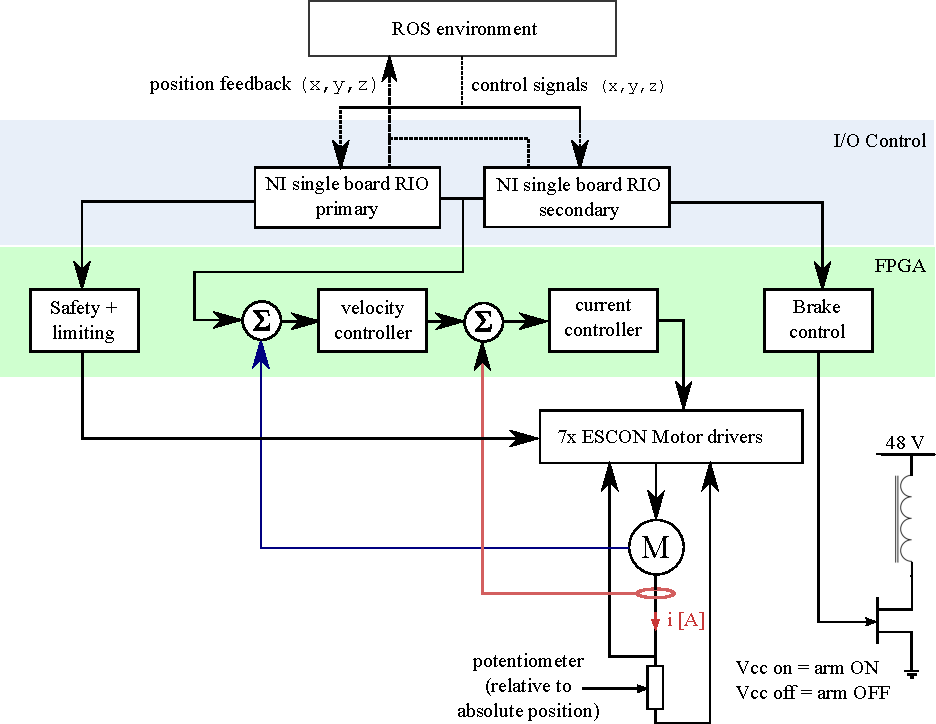
\includegraphics[width=0.95\textwidth]{overview.pdf}	\caption{This is a nice figure. Here illustrated for hand roll master.}
	\label{fig:overview}
\end{figure}
The focus of this thesis is the highest abstraction layer, i.e.the ROS environment. The purpose here primary constitute implementation of:
\begin{itemize}
\item Everything that require heavy processing \citep{bib:robot_paper}.
\item Non real-time processing or tasks with loose timing constraints \citep{bib:robot_paper}.
\end{itemize}
The above pool of stipulations will essentially and practically entail the following main topics of this thesis:
\begin{itemize}
\item All user interaction
\item Positioning control loops
\item Path planning
\end{itemize}
A crucial matter when dealing with those topics within robotic surgeries feature necessary conditions to guarantee the patient safety and to avert patient trauma \citep{bib:safety}.
\section{Safety Precautions for Automated Surgery Control}
The definition of safety will follow the definition described in \citep{bib:safety}, i.e.:
\begin{exa}
A closed loop control system, $\Gamma_\text{cl} = (f_\text{cl},h,X,X_0.X_u,D)$, is unsafe if there exist a time $t \in [0,T]$ such that the trajectory $\phi_{X_0}^{\bar{d}} : [0,T]$ satisfy: 
	\begin{flalign*}
		\left( \phi_{X_0}^{\bar{d}}([0,t]) \cap X_u \right) \neq \emptyset \kk \wedge \kk 
		\phi_{X_0}^{\bar{d}}([0,t]) \subseteq X
	\end{flalign*}
The closed loop system $\Gamma_\text{cl}$ is safe if there are no unsafe trajectories.
\label{def_safety}
\end{exa}
A graphical interpretation can be deduced from \autoref{def_safety} and found in figure ??.
\section{Control Barrier Functions}
The control of the safety problem can be carried out by inspiration of ordinary CLFs (Control Lyapunov Functions) \citep{bib:org_control}